\chapter{Stochastic optimal power flow (SOPFLOW)}\label{chap:sopflow}
SOPFLOW solves a stochastic security-constrained multi-period optimal power flow problem. The problem is set up as a two-stage optimization problem where the first-stage (base-case) represents the normal operation of the grid (or the most likely forecast) and the second-stage comprises of $N_s$ scenarios of forecast deviation. Each scenario can have multiple contingencies and each contingency can be multi-period. Thus, depending on the options selected, each stochastic scenario can be
\begin{itemize}
    \item Single-period, no contingency
    \item Single-period contingencies
    \item Multi-period contingencies
\end{itemize}

\section{Formulation}
An illustration of \sopflow in Fig. \ref{fig:sctopflow} for a case with two scenarios $s_0$ and $s_1$. Each scenario has two contingencies $c_0$, $c_1$, and each contingency has four time-periods.

\definecolor{lavander}{cmyk}{0,0.48,0,0}
\definecolor{violet}{cmyk}{0.79,0.88,0,0}
\definecolor{burntorange}{cmyk}{0,0.52,1,0}

\def\lav{lavander!90}
\def\oran{orange!30}

\tikzstyle{time}=[draw,circle,violet,bottom color=\lav,
                  top color= white, text=violet,minimum width=20pt]
                  
\tikzstyle{base}=[draw,circle,burntorange, left color=\oran,
                       text=violet,minimum width=20pt]

\begin{figure}[h!]
\centering
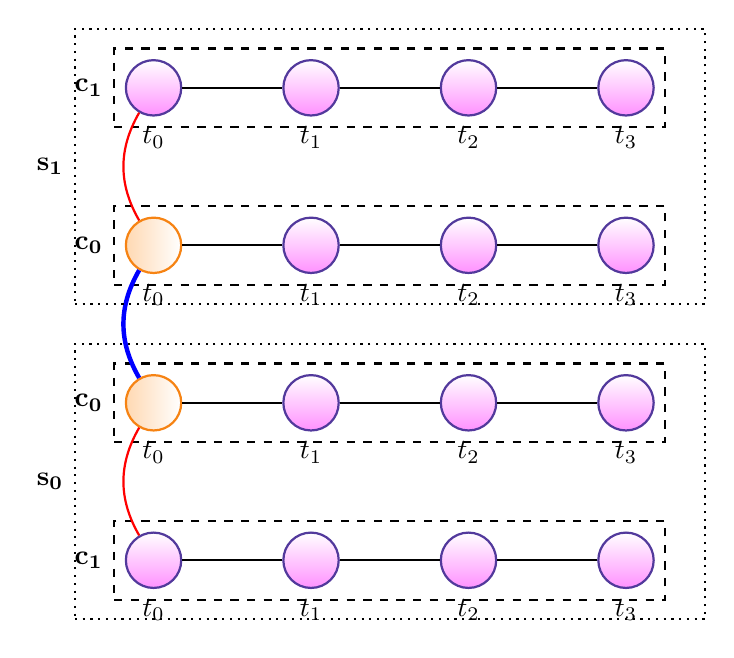
\begin{tikzpicture}[auto, thick]
  % scenario 0
  \node[base,label=below:$t_0$] (s0c0t0) at (0,2) {};
  \node[time,label=below:$t_1$] (s0c0t1) at (2,2) {};
  \node[time,label=below:$t_2$] (s0c0t2) at (4,2) {};
  \node[time,label=below:$t_3$] (s0c0t3) at (6,2) {};
  
  \path (s0c0t0) edge (s0c0t1);
  \path (s0c0t1) edge (s0c0t2);
  \path (s0c0t2) edge (s0c0t3);
  
  % contingency rectangle from (-0.5,1.5) to (6.5,2.5)
   \node[draw,rectangle,dashed,minimum width=7cm,minimum height=1cm,label=left:{$\mathbf{c_0}$}] (s0) at (3.0,2.0) {};
  
  \node[time,label=below:$t_0$] (s0c1t0) at (0,0) {};
  \node[time,label=below:$t_1$] (s0c1t1) at (2,0) {};
  \node[time,label=below:$t_2$] (s0c1t2) at (4,0) {};
  \node[time,label=below:$t_3$] (s0c1t3) at (6,0) {};
  
  \path (s0c1t0) edge (s0c1t1);
  \path (s0c1t1) edge (s0c1t2);
  \path (s0c1t2) edge (s0c1t3);
  
  % contingency rectangle from (-0.5,-0.5) to (6.5,0.5)
   \node[draw,rectangle,dashed,minimum width=7cm,minimum height=1cm,label=left:{$\mathbf{c_1}$}] (s0) at (3.0,0.0) {};
  
   \path (s0c0t0) edge [bend right,color=red] (s0c1t0);
  
  % scenario rectangle from (-1.0,-0.75) to (7.0,2.75)
   \node[draw,rectangle,dotted,minimum width=8cm,minimum height=3.5cm,label=left:{$\mathbf{s_0}$}] (s0) at (3.0,1.0) {}; 
  
  % scenario 1
  \node[base,label=below:$t_0$] (s1c0t0) at (0,4) {};
  \node[time,label=below:$t_1$] (s1c0t1) at (2,4) {};
  \node[time,label=below:$t_2$] (s1c0t2) at (4,4) {};
  \node[time,label=below:$t_3$] (s1c0t3) at (6,4) {};
  
  \path (s1c0t0) edge (s1c0t1);
  \path (s1c0t1) edge (s1c0t2);
  \path (s1c0t2) edge (s1c0t3);
  
   % contingency rectangle from (-0.5,3.5) to (6.5,4.5)
   \node[draw,rectangle,dashed,minimum width=7cm,minimum height=1cm,label=left:{$\mathbf{c_0}$}] (s0) at (3.0,4.0) {};
  
  \node[time,label=below:$t_0$] (s1c1t0) at (0,6) {};
  \node[time,label=below:$t_1$] (s1c1t1) at (2,6) {};
  \node[time,label=below:$t_2$] (s1c1t2) at (4,6) {};
  \node[time,label=below:$t_3$] (s1c1t3) at (6,6) {};
  
  \path (s1c1t0) edge (s1c1t1);
  \path (s1c1t1) edge (s1c1t2);
  \path (s1c1t2) edge (s1c1t3);
  
   % contingency rectangle from (-0.5,5.5) to (6.5,6.5)
   \node[draw,rectangle,dashed,minimum width=7cm,minimum height=1cm,label=left:{$\mathbf{c_1}$}] (s0) at (3.0,6.0) {};
  
  \path (s1c0t0) edge [bend left,color=red] (s1c1t0);
  
  \path (s0c0t0) edge [bend left,ultra thick,color=blue] (s1c0t0);
  
   % scenario rectangle from (-1.0,3.75) to (7.0,6.75)
   \node[draw,rectangle,dotted,minimum width=8cm,minimum height=3.5cm,label=left:{$\mathbf{s_1}$}] (s1) at (3.0,5.0) {};
  

\end{tikzpicture}
\caption{Stochastic multi-period contingency constrained example with two scenarios $s_0$ and $s_1$. Each scenario has two contingencies $c_0$,$c_1$ and each contingency consists of four time-periods $t_0$, $t_1$, $t_2$, $t_3$. State $s_0,c_0,t_0$ represent the base case (no contingency) case for the two scenarios.  We assume that any contingency is incident at the first time-step, i.e., at $t_0$. Thus, the contingency states $c_1,t_0$ is coupled with the no-contingency state $c_0,t_0$ at time $t_0$ for both the scenarios. The {\textcolor{red}{red}} line denotes the coupling between the contingency and the no-contingency states.The {\textcolor{blue}{blue}} line denotes the coupling between the scenarios}
\label{fig:sctopflow}
\end{figure}

The formulation for the stochastic security-constrained multi-period optimal power flow is given in (\ref{eq:sctopflow_start}) -- (\ref{eq:sctopflow_end}). In this formulation, the objective is to reduce the expected cost, where $f(x_{s,0,0})$ is the cost for scenario $s$ with no contingencies (hence 0 for the contingency index). $\rho_s$ is the probability of scenario $s$.

\begin{align}
\centering
\text{min}&~\sum_{s=1}^{N_s-1}\pi_s\sum_{c=0}^{N_c-1}\sum_{t=0}^{N_t-1}f(x_{s,c,t})&  \label{eq:sctopflow_start}\\
&\text{s.t.}& \nonumber \\
&~g(x_{s,c,t}) = 0,                                        &s \in \left[1,N_s-1\right],c \in \left[0,N_c-1\right], t \in \left[0,N_t-1\right]& \\
&~h(x_{s,c,t}) \le 0,                                      &s \in \left[1,N_s-1\right],c \in \left[0,N_c-1\right], t \in \left[0,N_t-1\right]& \\
x^- & \le x_{s,c,t} \le x^+,                               &s \in \left[1,N_s-1\right],c \in \left[0,N_c-1\right], t\in \left[0,N_t-1\right]& \\
-\delta_t{x} & \le x_{s,c,t} - x_{s,c,t-\Delta{t}} \le \delta_t{x},&s \in \left[1,N_s-1\right],c \in \left[0,N_c-1\right], t \in \left[1,N_t-1\right]& \label{eq:sctopflow_time_coupling}\\
-\delta_c{x} & \le x_{s,c,0} - x_{s,0,0} \le \delta_c{x},&s \in \left[1,N_s-1\right],c \in \left[1,N_c-1\right]&
\label{eq:sctopflow_contingency_coupling} \\
-\delta_s{x} & \le x_{s,0,0} - x_{0,0,0} \le \delta_s{x},&s \in \left[1,N_s-1\right]&
\label{eq:sctopflow_end}
\end{align}

{\sopflow} uses all the modeling details used for modeling an optimal power flow problem, i.e., each of the circles shown in Fig. \ref{fig:sctopflow} has the modeling details of an optimal power flow problem (\opflow). Incorporating the probabilities $\pi_s$ for each scenario is not implemented yet which leads to each scenario having an equal probability. 

Currently, \sopflow uses wind power generation as the stochastic variables and each scenario is a realization of the power output from wind generators. A zero fuel cost is used for wind power generation to ensure wind generation would be the dispatched to the given target level (upper limit). 

For contingencies, \sopflow supports generation and/or transmission outages. A contingency can have multiple outages, but, it should not cause any islanding. The coupling between the no-contingency and the contingency case for each scenario is also the difference in real power output ($p_{jsct}^{\text{g}} - p_{js0t}^{\text{g}},~ \jinJgen$) that must be within the 30 minute generator ramp rate.

For multi time-period, we use ramping constraints on the generator real power output between successive time steps.

\sopflow can be run in two modes: preventive and corrective. In the preventive mode, generator real power output is fixed to the base-case values for generators at PV bus(es). In this mode, the generators at the reference bus provide/absorb any deficit/surplus power. The corrective mode allows deviation of the PV and PQ generator real power from the base-case dispatch constrained by its 30-min. ramp rate capability. Note that the preventive/corrective mode is only applied at the first step $t_0$. In the successive time-steps, the generator dispatch is dictated by the previous step dispatch and the ramp limits.

\section{Solvers}
\sopflow can be solved with \ipopt. If one wants to solve each scenario independently, i.e., without any coupling constraints then use \emph{EMPAR} solver. \emph{EMPAR} distributes the contingencies to different processes when executed in parallel.

\section{Input and Output}
The following files are needed for executing a SOPFLOW.
\begin{itemize}
    \item \textbf{Network file:} The network file describing the network details. Only \matpower format files are currently supported.
    \item \textbf{Scenario file:} \sopflow only supports reading wind generation scenarios in a CSV format. An example of this format for the 9-bus case is \href{https://gitlab.pnnl.gov/exasgd/frameworks/exago/-/tree/master/datafiles/case9/scenarios.csv}{here}.
    \item \textbf{Contingency file:} Contingencies can be specified via PTI format file as described in chapter \ref{chap:scopflow}.The option \lstinline{-sopflow_enable_multicontingency} should be set for multi-contingency problems.
    \item \textbf{Load data:} One file for load real power and one fo reactive power. The files need to be in CSV format. An example of the format for the 9-bus case is \href{https://gitlab.pnnl.gov/exasgd/frameworks/exago/-/tree/master/datafiles/case9}{here}.
\end{itemize}

The \sopflow output is saved to a directory named \emph{sopflowout}. This directory contains $N_s$ subdirectories to save the solution for each scenario. Each of these subdirectories contain $N_c$ subdirectories, one for each contingency. Each contingency subdirectory has $N_t$ MATPOWER format files to store the output for each time-period for the given contingency and scenario. The subdirectories have the directory name format \emph{scen\_x} where x is the scenario number,  \emph{cont\_y} where y is the contingency number, and the output files have the file name format \emph{t\_z} where z is the time-step number.

\section{Usage}
\begin{lstlisting}
    ./sopflow -netfile <netfilename>  -scenfile <scenfilename> <sopflowoptions>
\end{lstlisting}
\todo

\section{Options}
See table \ref{tab:sopflow_options}

\begin{table}[!htbp]
  \caption{SOPFLOW options}
  \small
  \begin{tabular}{|p{0.4\textwidth}|p{0.3\textwidth}|p{0.3\textwidth}|}
    \hline
    \textbf{Option} & \textbf{Meaning} & \textbf{Values (Default value)} \\ \hline
    -netfile & Network file name & string (\href{https://gitlab.pnnl.gov/exasgd/frameworks/exago/-/blob/master/datafiles/case9/case9mod_gen3_wind.m}{case9mod_gen3_wind.m}) \\ \hline
    -scenfile & Scenario file naame & string (\href{https://gitlab.pnnl.gov/exasgd/frameworks/exago/-/blob/master/datafiles/case9/scenarios.csv}{scenarios.csv}) \\ \hline
    -sopflow\_mode & Operation mode: Preventive or corrective & 0 or 1 (0) \\ \hline
    -sopflow\_enable\_multicontingency & Multi-contingency SOPFLOW & TRUE or FALSE (FALSE) \\ \hline 
  \end{tabular}
  \label{tab:sopflow_options}
\end{table}

With multi-contingency SOPFLOW, all \scopflow options given in Table \ref{tab:scopflow_options} can be used to tune the contingencies.

Depending on the \emph{mode}, SOPFLOW can either be \emph{preventive} (mode = 0) or \emph{corrective} (mode = 1). In the preventive mode, the PV and PQ generator real power is fixed to its corresponding base-case values. The generators at the reference bus pick up any make-up power required for the contingency. The corrective mode allows deviation of the PV and PQ generator real power from the base-case dispatch constrained by its 30-min. ramp rate capability.

\section{Examples}
\todo
